%! Author = sbbfti
%! Date = 10/06/2020

\section{Methodology}\label{sec:methodology}

% todo the set model has the issue with the fact that it iterates over that strange parameter lenght of time = 6o

In this manuscript, we used the heat balance model that \mycite{GaggeSET} developed to derive the \ac{set} to determine when the use of elevated air moment (e.g.. \ac{v} $>$ 0.2 m/s) would be beneficial to cool the human body.
% todo say something that v is the average air speed and not the speed of the air coming out from the fan
The heat balance model allows us to estimate how environmental (i.e., \ac{t-db}, \ac{t-r}, \ac{v}, \ac{rh}) and personal factors (i.e., \ac{clo}, \ac{met}) influence both latent and sensible components of the \ac{q-sk}, and the \ac{q-res}.
Moreover, it can be used to estimate the value of some physiological variables such as, \ac{t-sk}, and \ac{t-cr}.

Section~\ref{subsec:energy-balance} describe the main Equations used by the model to derive the results.
We have published the algorithm we used to calculate the results in a public repository.
% todo add link to repository
% todo say that Gagge's equation is written in a un-used language, hence we have converted it to Python and JavaScript
Moreover, we added it to the pythermalcomfort Python package~\cite{Tartarini2020a} and the CBE thermal comfort tool~\cite{Tartarini2020}.
The former can be used by Python users to calculate the results presented in this manuscript.
The latter is a web-based tool that can be used to generate interactive figures which show the environmental conditions under which the use of elevated air speeds is beneficial.

\subsection{Energy Balance}\label{subsec:energy-balance}

The human body exchanges both sensible and latent heat with its surrounding environment.
Sensible heat is transferred via conduction, convection and radiation (\acs{c-r} + \acs{c-res}).
While latent heat losses occur from evaporation of sweat  (\acs{e-rsw}), moisture diffused through the skin  (\acs{e-dif}), and respiration (\acs{e-res})
The energy balance in the human body is described by:

\begin{equation}
    M - W = (C + R + E_{sk}) + (C_{res} + E_{res}) + (S_{sk} + S_{cr})\label{eq:heat-balance}
\end{equation}

This equation assumes that the body comprises two main thermal compartments: the skin and the core.
If the exogenous and endogenous heat gains cannot be compensated by the heat losses, then both the \ac{s-sk}, and the \ac{s-cr} increase and in turn the \ac{t-sk}, and \ac{t-cr} rise, respectively.

The amount of sensible heat gains or losses from the human body to its environment can be expressed as a function of environmental, and personal factors.
The former are \ac{t-db}, \ac{t-r}, \ac{v}, and \ac{rh}.
While the latter are \ac{met}, and \ac{clo}~\cite{ASHRA2017}.

The equations used to determine sensible and latent heat loss are based on fundamental heat transfer theory, while the coefficient were estimated empirically~\cite{ASHRA2017}.

\subsubsection{Body Surface Area, (\acs{body-a})}

All the terms presented in Equation~\ref{eq:heat-balance} are reported in power per unit of human \ac{body-a}.
Equation~\ref{eq:dubois} can be used to estimate \ac{body-a} as a function of the \ac{body-w} and \ac{body-h} of the person~\cite{DuBois}.

\begin{equation}
    A_{body} = 0.202 m^{0.425} l^{0.725}\label{eq:dubois}
\end{equation}

% look at this source

\subsubsection{Sensible Heat Loss from Skin, (\acs{c-r})}

Sensible heat losses from the human body mainly occur from convection and radiation from the skin to the environment.
The total amount of \ac{c-r} can be described as a function of the \ac{t-sk}, \ac{t-op}, \ac{r-cl}, \ac{f-cl}, and \ac{h}.
The equation can be expressed as:

\begin{equation}
    C+R=\frac{t_{s k}-t_{o}}{R_{c l}+1 /\left(f_{c l} h\right)}\label{eq:c-r}
\end{equation}

\begin{equation}
    f_{cl}=1.0 + 0.31 I_{cl} \label{eq:f-cl}
\end{equation}

\begin{equation}
    h=h_{c} + h_{r} = \max(3, 8.6 v^{0.53}) p_{atm}^{0.53} + 4 \varepsilon \sigma \frac{A_{\mathrm{r}}}{A_{body}}\left[273.2+\frac{\left(t_{\mathrm{cl}}+\overline{t_{r}}\right)}{2}\right]^{3}\label{eq:h}
\end{equation}

% todo describe variables that did not appear in the text before

Where \ac{t-op} varies as a function of \ac{h-c}, \ac{h-r}, \ac{t-r} and \ac{t-db}, and it is described by:

\begin{equation}
    t_{o}=\frac{h_{r} \bar{t}_{r}+h_{c} t_{db}}{h_{r}+h_{c}}\label{eq:t-op}
\end{equation}

The \ac{t-sk} is calculated iteratively by the heat balance model since it varies as a function of the heat loss from the human body towards its environment and the heat transferred from the core to the skin node.
\Ac{t-cl} can be calculated as a function of the \ac{t-op}, \ac{t-sk}, \ac{r-cl} and the resistance of the air layer.

\subsubsection{Latent Heat Loss from Skin, (\acs{e-sk})}

The \acf{e-sk} comprises two terms the \ac{e-rsw} and the \ac{e-dif}.
\ac{e-sk} depends on the \ac{w}, \ac{p-sk} normally assumed to be that of saturated water vapor at \ac{t-sk}, \ac{p-a}, \ac{f-cl}, \ac{h-e}, and \ac{r-e-cl}.

\begin{equation}
    E_{s k}=E_{rsw}+E_{dif}=\frac{w\left(p_{s k, s}-p_{a}\right)}{R_{e, c l}+1 /\left(f_{c l} h_{e}\right)}\label{eq:latent-skin}
\end{equation}

Despite the fact that Equation~\ref{eq:latent-skin} is expressed as a function of \ac{w}.
The human body does not regulates \ac{w} directly but, rather, it regulates the sweat rate~\cite{ASHRA2017}.
Skin wettedness varies as a function of the activity of the sweat glands and the environmental conditions~\cite{ASHRA2017}.
While, theoretically \ac{w} can range from 0 to 1, in practice, \ac{w} is strongly correlated with thermal stress and warm discomfort, consequently there is a \ac{w-max} for sustained activity for healthy and acclimatized humans~\cite{ASHRA2017}.

We estimated the \ac{w-max} value and the \ac{m-sweat} using the \mycite{GaggeSET} model.

\subsubsection{Respiratory Losses, (\acs{q-res})}
The human body exchanges both sensible and latent heat with its environment.
The \acf{q-res} equals the sum of the \ac{c-res} and the \ac{e-res}.
The value of \ac{q-res} is can be determined using the following simplified equation~\cite{ASHRA2017}:

\begin{equation}
    q_{res} = C_{res} + E_{res} = 0.0014M(34-t_{a}) + 0.0173M(5.87-p_{a})\label{eq:respiratory-losses}
\end{equation}

\subsection{Data Analysis}\label{subsec:data-analysis}

The heat balance model was used to estimate the sensible and latent heat loss and physiological parameters (e.g., \ac{m-sweat}, \ac{t-cr}).
We calculated the results for \ac{t-op} ranging from 28 and 55~$^{\circ}$C at 0.5~$^{\circ}$C intervals, \ac{rh} ranging from 0 to 100~\% at 5~\% intervals and for the discrete values of \ac{v} = 0.2, 0.8 and 4.5~m/s.
In this paper we will be referring to `still air' condition when air velocities are below \ac{v}~=~0.2 m/s.
This definition is in accordance with the ASHRAE 55--2017 Standard~\cite{ashrae552017} and allowed us to compare our results with~\mycite{Jay2015}.
We assumed \ac{t-r} to be equal to \ac{t-db}, \ac{clo}~=~0.5 clo, and \ac{met}~=~1.0 met, unless otherwise stated.
It could be argued that \ac{clo} of people during heatwaves may be even lower than 0.36 clo (i.e., walking shorts, short-sleeve shirt and sandals), however, we wanted to consider a conservative scenario.
Results for different combinations of environmental and personal conditions can be generated using our online tool.
We reported heat loss per unit of surface area (i.e., \ac{e-sk}).
To obtain the absolute value of heat loss or gain the results can be multiplied by \ac{body-a}.
Thermal stress was assumed to occur when \ac{w} (which only depends on the value of \ac{v}) reaches its maximum value \ac{w-max}.
We assumed that the use of electrical fans is detrimental when the value of \ac{t-cr} calculated for values of \ac{v} higher than 0.2~m/s exceeds the value determined for the `still air' condition.

\subsection{Weather data}\label{subsec:weather-data}

The results obtained with the proposed heat balance model were compared with the climatic data provided in the 2017 ASHRAE Handbook--Fundamentals~\cite{ASHRA2017}.
We used the ASHRAE climatic design database to extract information regarding the maximum extreme dry-bulb and wet-bulb temperatures recorded across more than 5000 stations worldwide over the last 50 years.
For more information about the ASHRAE climate database please refer to Chapter 14 of the 2017 ASHRAE Handbook--Fundamentals.
Maximum extreme dry-bulb temperatures are shown in Figure~\ref{fig:world-map}, in which we present data from all the stations with values higher than 20 $^\circ$C\@.

\begin{figure}[thb!]
    \centering
    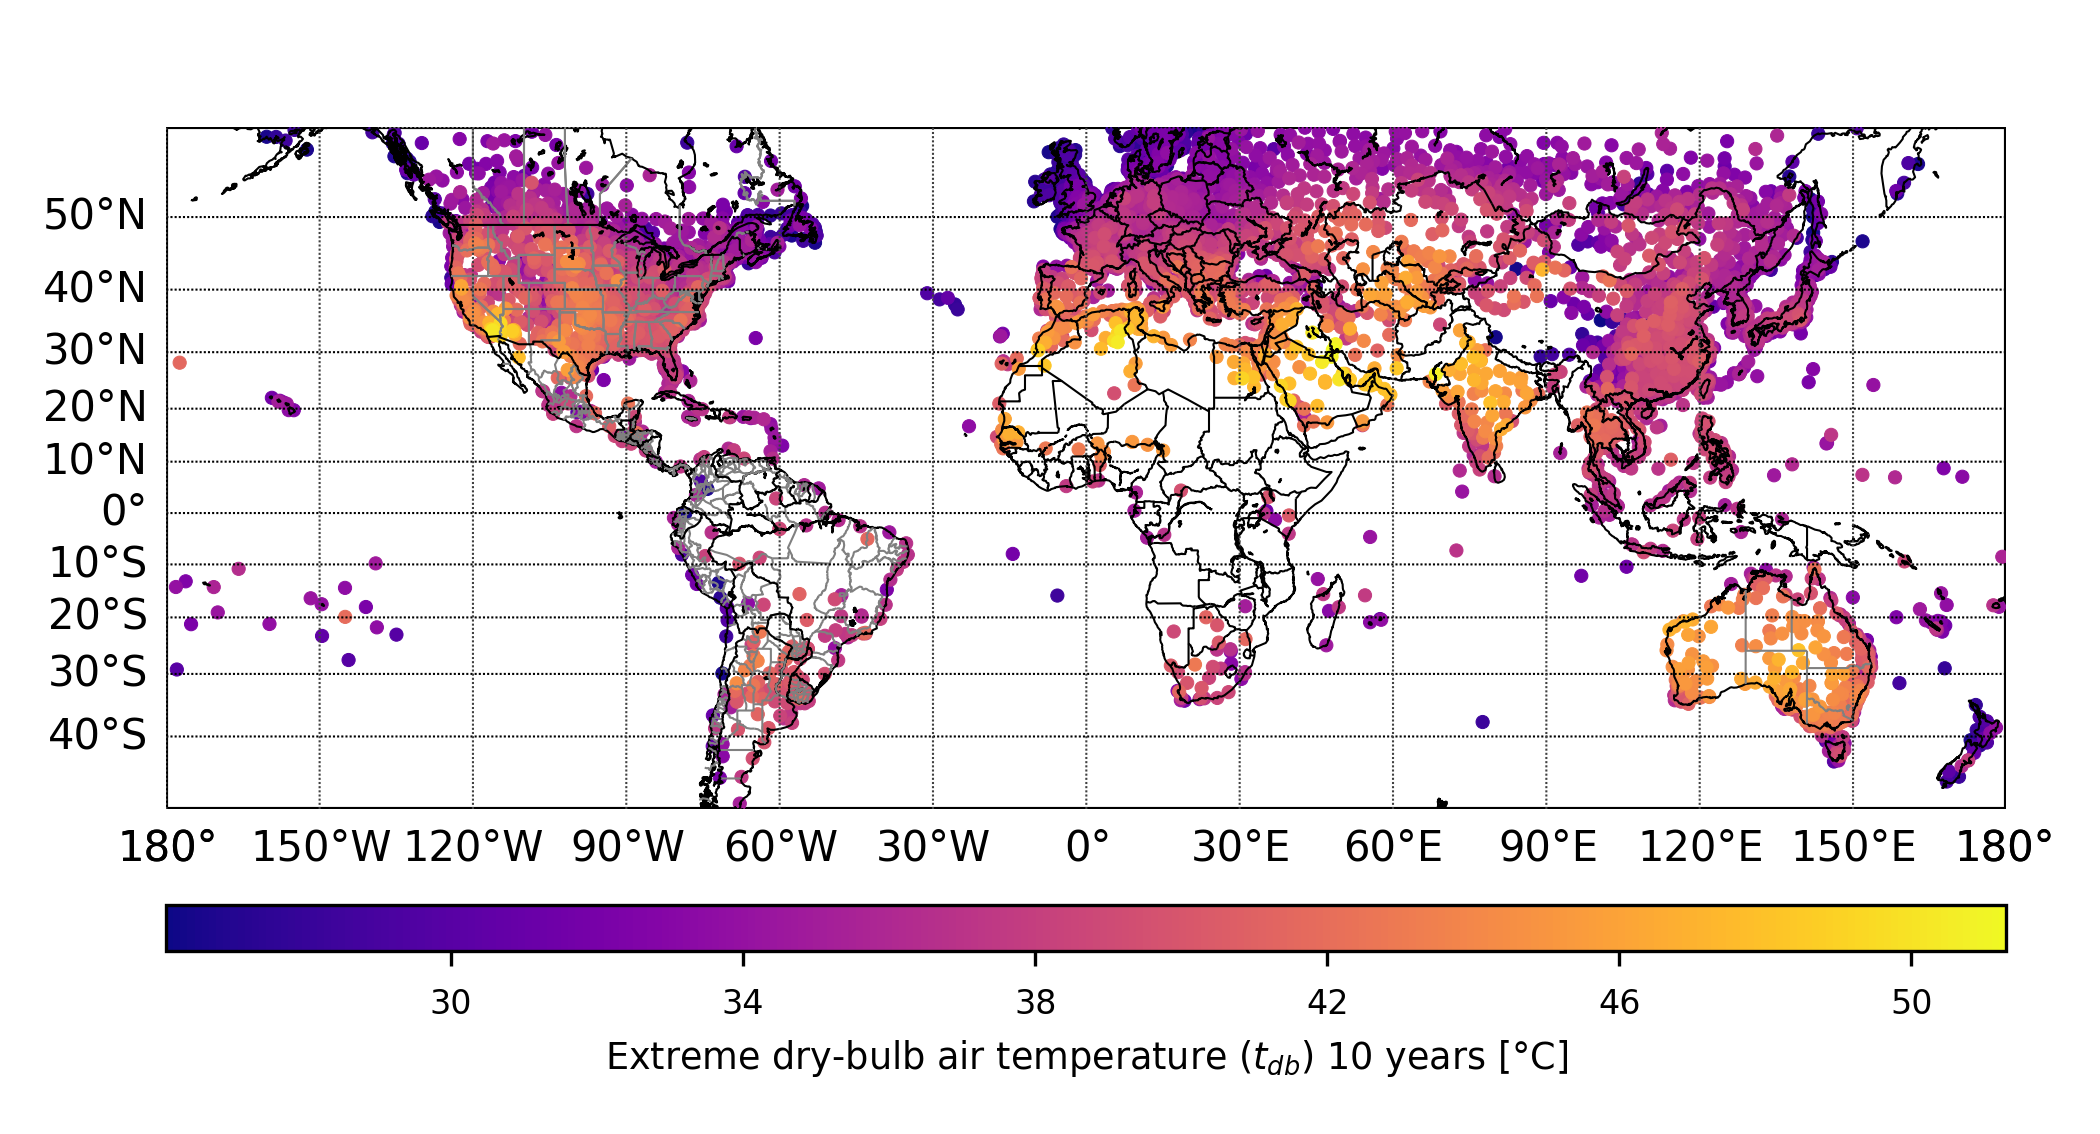
\includegraphics[width=\textwidth]{figures/world-map.png}
    \caption{Shows the location of each weather station that was included in the analysis and the maximum extreme dry-bulb temperature that was recorded in that location over the last 50 years.}
    \label{fig:world-map}
\end{figure}

The five highest dry-bulb air temperatures were recorded in Morocco, USA, Iran, Algeria and Saudi Arabia, while the five highest wet-bulb air temperatures were all recorded in Australia.
Figure~\ref{fig:world-map} also shows that few data was available for the Sub-Saharan Africa where approximately 40\% of the poorest people in the world reside and where climate change may be an acute threat~\cite{PovertyO1:online}.

\subsection{Elderly}

% todo say something how we calculated w for the elderly

\subsection{Open-source tools}

% todo descibe the CBE tool and pythermalcomfort equation to generate the figures